\documentclass[12pt, openany]{book}
\usepackage{graphicx}
\usepackage{tikz}
\usetikzlibrary{spy}


% This is all the packages and settings and so on.
% It is using custom fonts that needs to be installed on the computer. If they are not present, they have to be added manually.
\usepackage[
	citestyle=ieee, 
    bibstyle=ieee,
    style=numeric-comp,
    sorting=nty,
    maxbibnames=99, % Make sure we are printing all authors in the appendix
    ]{biblatex}
    
% Makes the last name first in the bibliography.
% \DeclareNameAlias{author}{last-first}
\DeclareNameAlias{author}{family-given}
    
% Specify the margins. This is 6.25inches in text with which 
% can be used to size figures to the correct size.
\usepackage[a4paper, margin=2.5625cm]{geometry}

\usepackage{eso-pic}					% Packages for layout and graphics 
\usepackage{graphicx}
\usepackage{tikz}
\usetikzlibrary{fadings}
\usepackage{setspace}
% \usepackage{tocloft}		 			% Fixing a bug with page style changes for toc
% \tocloftpagestyle{plain}
\usepackage{etoc} 						% Separate tocs for appendix and the rest    
\usepackage{chngcntr}					% Count figures within chapters
\usepackage{booktabs}					% Table formatting
\usepackage{fancyhdr}					% Setting the style for header and footer.
\usepackage{tabularx}
\usepackage{multirow}                   % For better tables 
\usepackage[hidelinks]{hyperref}		% Clickable links
\usepackage{nameref}					% References with names
\usepackage[parfill]{parskip}			% New line instead of indent for sections
\usepackage{tcolorbox}					% Create boxes around content
\tcbset{colback=white,arc=0mm}

\usepackage{amsmath}
\usepackage{mathdots}
\usepackage{yhmath}
\usepackage{siunitx}
\usepackage{array}
\usepackage{gensymb}
\usepackage{amssymb}
\usepackage{mathtools}              % Add text to math arrows.

\usepackage{cancel}
\usepackage{color}
\usepackage{multirow}
\usepackage{textcomp}               % Fixing warning for gensyb \perthousand
\usepackage{svg}                    % including svg files
\usepackage{caption}                % For subfigures
\usepackage{subcaption}
\usepackage{fontspec}
\usepackage{sectsty}
\usepackage{tocloft}

\usepackage[printonlyused]{acronym}


\counterwithin{figure}{section} 
\counterwithin{table}{section}

% Specifying fonts
\setmainfont{Georgia} 
\setsansfont{Arial}
\newfontfamily\footerfont{Georgia}

\chapterfont{\sffamily\fontsize{17}{17}}
\sectionfont{\sffamily\fontsize{14}{15}}
\subsectionfont{\sffamily\fontsize{13}{15}}
\subsubsectionfont{\sffamily\fontsize{12}{15}}

% Remove the title and make sure that the text is adjusted
% \usepackage{abstract}
% \setlength{\absleftindent}{0mm}
% \renewcommand{\abstractname}{\vspace{-\baselineskip}}
% \renewcommand{\abstractnamefont}{\sffamily\fontsize{14}{15}}
% \renewcommand{\abstracttextfont}{\normalfont\fontsize{12}{13}}

% Renaming and setting style of table of contents
\renewcommand*\contentsname{Contents}
\renewcommand*\cfttoctitlefont{\fontsize{16}{0}\bf\sffamily}
\renewcommand\cftchapfont{\fontsize{14}{0}\bf\sffamily}
\renewcommand\cftchappagefont{\fontsize{13}{0}\bf\sffamily}
\renewcommand\cftsecfont{\fontsize{12}{0}\sffamily}
\renewcommand\cftsecpagefont{\fontsize{12}{0}\sffamily}
\renewcommand\cftsubsecfont{\fontsize{12}{0}\sffamily}
\renewcommand\cftsubsecpagefont{\fontsize{12}{0}\sffamily}

% Styling the header and footer
\fancyhf{}
\fancyhead{}
\fancyfoot{}
\fancyhead[L]{\fontsize{11}{10}\selectfont\leftmark}
\fancyfoot[R]{\footerfont\thepage}
\setlength{\headheight}{15.5pt}


\fancypagestyle{plain}{
    \fancyhf{}
    \fancyhead{}
    \fancyfoot{}
    \renewcommand{\headrulewidth}{0pt}
    \fancyfoot[R]{\footerfont\thepage}
}

\pagestyle{fancy}

% Making the command for placing text in random locations
\newcommand\PlaceText[3]{%
\begin{tikzpicture}[remember picture,overlay]
\node[outer sep=0pt,inner sep=0pt,anchor=south west] 
  at ([xshift=#1,yshift=-#2]current page.north west) {#3};
\end{tikzpicture}%
}

% Disable hyphenation
\pretolerance=10000
\tolerance=2000 
\emergencystretch=50pt


% Defining files for bibliography
%\addbibresource{ref.bib}
\addbibresource{references.bib}
% Add a second bibliography file for the second author to allow
% both to update it through the mendeley integration.
% \addbibresource{ref-author-2.bib}

% Defining document information
\title{Remote Sensing-based Socioeconomic Analysis using Transfer Learning and Ridge Regression}
\newcommand{\subtitle}{Project Report}
\author{<Author Name and Author Name>}

\begin{document}
\setstretch{1.4}

% The front page of the document
\pagenumbering{roman}
\makeatletter
\begin{titlepage}

\vspace*{-4.6\baselineskip}
x\hspace*{-0.15\textwidth}
\includegraphics[width=0.3\paperwidth]{setup/img/lakehead_logopng.png}
\par\vspace*{2.5\baselineskip}

\PlaceText{65mm}{12mm}{\fontsize{12}{0}\sffamily MASTERS IN COMPUTER SCIENCE,}
\PlaceText{65mm}{17mm}{\fontsize{12}{0}\sffamily DEPARTMENT OF COMPUTER SCIENCE,}
\PlaceText{65mm}{22mm}{\fontsize{12}{0}\sffamily\itshape 955 Oliver Rd, Thunder Bay, ON P7B 5E1, CANADA \the\year}

~\\

\makebox[0pt][l]{%
\begin{minipage}[b]{0.25\textwidth}
~\\
\end{minipage}
\begin{minipage}{0.65\textwidth}
\begin{flushleft}
{\fontsize{28}{24}\bf\sffamily\@h Remote Sensing-based Socioeconomic Analysis using Transfer Learning and Regression}\\
\vspace{1cm}
{\fontsize{20}{18}\bf\sffamily \@h Project Report}
\vspace{1cm} \\
%{\fontsize{16}{18}\sffamily \@h Sree Teja Buddaraju, Ananya Bardhan, Ramya Sri Boddu, Simranjit Kaur, Thangarajah~Akilan,~\IEEEmembership{Member,~IEEE}}
\\
\end{flushleft}
\end{minipage}
}



% \hspace*{-3cm}\begin{minipage}[b]{63.5mm}
% ~\\
% \end{minipage}
% \begin{minipage}{0.65\textwidth}
% \begin{flushleft}
% {\fontsize{28}{24}\bf\sffamily\@title\\}
% \vspace{0.5cm}
% {\fontsize{19}{17}\bf\sffamily \subtitle\\}
% \vspace{0.5cm} 
% {\fontsize{16}{0}\sffamily \@author}\\
% \end{flushleft}
% \end{minipage}


\AddToShipoutPictureBG*{%]
    \AtPageLowerLeft{%
        \includegraphics[width=1.0\paperwidth]{setup/img/kth-footer.png}
    }%
}

\PlaceText{70mm}{280mm}{\color{white}\fontsize{12}{0}\sffamily LAKEHEAD UNIVERSITY }
\PlaceText{70mm}{285mm}{\color{white}\fontsize{8}{0}\sffamily DEPARTMENT OF COMPUTER SCIENCE }
\end{titlepage}
\makeatother

\newpage
\newpage
\thispagestyle{plain}
~\\
\vfill
{ \setstretch{1.1}
	\subsection*{Authors}
	Sree Teja Buddaraju  \\ Ananya Bardhan \\
	Ramya Sri Boddu \\
	Simranjit Kaur \\

	\subsection*{Supervisor}
	Dr. Thangarajah Akilan\\
% 	Thunder Bay, Ontario\\
% 	Lakehead University
	
	\subsection*{Place for Project}
	Department of Computer Science\\
	Lakehead University\\
	955 Oliver Rd, Thunder Bay, ON P7B 5E1\\
	Canada
	~
%	\subsection*{Examiner}
%	The Professor
%	Place \\
%	KTH Royal Institute of Technology
	

}


\newpage
\thispagestyle{plain}
%%%%%%%%%%%%%%%%%%%%%%%%%%%%%%%%%%%%
%%  The English abstract          %%
%%%%%%%%%%%%%%%%%%%%%%%%%%%%%%%%%%%%
\chapter*{Abstract}
%%%%%%%%%%%%%%%%%%%%%%%%%%%%%%%%%%%%


\vspace{0.5cm}
The economic status of each country varies. Some countries are well developed while some are underdeveloped. A lower economic status in any state can lead to hunger, malnutrition, and low life expectancy of the people living there, especially for children and the older generation. Most of them live below the international poverty line of 1.25 US dollar per day according to the World Bank Group. One way of working towards solving this problem is through collecting information for analysis which works as a vital resource for the organizations that can help the people there to lead a better life. But obtaining this information in the conventional way through human surveys takes too long and requires a lot of resources. This work is intended to act as an alternative to this problem, it analyzes the social and economic status of the underdeveloped countries, primarily the selected African countries, by exploiting machine learning and image processing technologies. This work proposes a set of algorithms that can make predictions on the standard of living of a particular geographic region based on the distribution of night lights observed through remote sensing and satellite image processing to provide more accurate results. This work is based on transfer learning where we train a model pre-trained on ImageNet and obtain predictions of the wealth distribution of a region using the data from National Oceanic And Atmospheric Administration (NOAA), Demographic and Health Survey (DHS), and Google static maps. The results show the performance analysis of the the models built, based on the correlation between the actual wealth as observed in the survey data and the wealth index predicted by the model. The predicted wealth is mapped on a heat map for visualizing the wealth distribution of the particular regions.




\subsection*{Keywords}
Remote sensing, Socioeconomic analysis, Machine learning







\newpage
\thispagestyle{plain}
\chapter*{Acknowledgements}
We would like to share  our sincere gratitude towards professor Dr. Thangarajan Akilan for actively supporting the idea behind this project and for his guidance and advice throughout its duration. We would like to thank our colleagues and peers who provided subjective measures to improve this project. 



\newpage
\chapter*{Acronyms}

\begin{acronym}[RDBMS]
%\acro{ACID}{atomicity, consistency, isolation, and durability}
%\acro{CAP}{Consistency, Availability, Partition-tolerant}
%\acro{CDF}{Cumulative Distribution Function}
\acro{DHS}{Demographic Health Survey}
\acro{NOAA}{National Oceanic and Atmospheric Administration}
\acro{NGDC}{National Geophysical Data Center}
\acro{EOG}{Earth Observation Group}
\acro{GDP}{Gross Domestic Product}
\acro{GDAL}{Geospatial Data Abstraction Library}
\acro{NGO}{Non Government Organization}
\acro{API}{Application Programming Interface}
\acro{CNN}{Convolution Neural Network}
\acro{PCA}{Principal Component Analysis}
\acro{MSE}{Mean Square Error}
\end{acronym}


\etocdepthtag.toc{mtchapter}
\etocsettagdepth{mtchapter}{subsection}
\etocsettagdepth{mtappendix}{none}
\thispagestyle{plain}
\tableofcontents

\newpage






\pagenumbering{arabic}


\chapter{Introduction}
Recent studies from Pew Research Centre have shown that a substantial amount of population from major African countries will be migrating in the next five years to Western and European countries for a better lifestyle which they are lacking in their country. Poverty is one of the most important factors to be looked at while deriving the economic status of a particular region\cite{jean2016combining}. Having a well formed data and record of poverty of a region can help the government and other organizations make informed decisions and implement certain policies that can work towards eradicating it. This can be done by collecting various kinds of data on the well being of the people of a particular place. Conducting surveys can be a method for data collection, but it is not practical in most of the regions as the accessibility is low, they tend to be expensive and time consuming. With the advancements of remote sensing, machine learning and image processing efficient predictive algorithms can be developed to analyze the socioeconomic factor of different regions and take precautionary actions before things get worse.

Battling the deficiency of reliable poverty data in the developing countries have been a challenge, hence there is a need for a cheap and scalable method of collecting such data to facilitate the economic progress in these areas. Some of the ways which can help in determining economic activity in vast geographic regions are:
\begin{itemize}
    

\item Night time luminous intensity using remote sensing.
\item Distribution of household structures and their parameters.
\item Automobile activity.
\end{itemize}

\section{Overview}
This chapter provides the information related to the work which includes background, the purpose, goal, methodology followed and the stakeholders of the project.

\section{Background}
\label{sec:background}


The economic status or livelihood is quite difficult to predict due to the scarcity of reliable data sets from various developing countries~\cite{jean2016combining}. Also topics like these are very crucial for both research and political purposes. In the recent years, though this kind of data has increased in quality and quantity due to widespread surveys being conducted and the emergence of new technologies which can capture the data easily. Even if this data gap exists, the \ac{DHS} program collects accurate data on health and population of developing countries. It provides us with valuable wealth distribution and household information in that region. It covers more than ninety countries worldwide now~\cite{mullainathan2017machine}.
 
The difficulties in collecting this data is that it requires a lot of human effort and lots of cost associated with it. Therefore, another reliable data source was needed. Hence a recent approach of using the satellite images of night light luminous intensity to predict the economic activity in the selected regions~\cite{pokhriyal2017combining}. These images taken from  \ac{NOAA} gives the stack of satellite images during night time captured during 8:30 PM to 10:30 PM. This visualization shows only the lights generated from electricity~\cite{jin2017method}.

Nightlight images do not expose geographical features, which can be found only on the Daytime captured satellite visuals giving a clear view of infrastructure, buildings, roads, farmland, etc. in a particular area. The Daytime satellite images are taken from Google Static Maps. The Google \ac{API} Key is required to download these images. They have a luminosity range of $0$ to $63$, where $0$ is no luminosity at all and $63$ being the most luminous and is spread across $1 km^2$ with a zoom level of $16$. As these are satellite images, only a little zooming will enlarge it to a great extent. Thus, this is the optimal value to be considered~\cite{chen2006remote}.


\begin{figure}[h!]
\centering
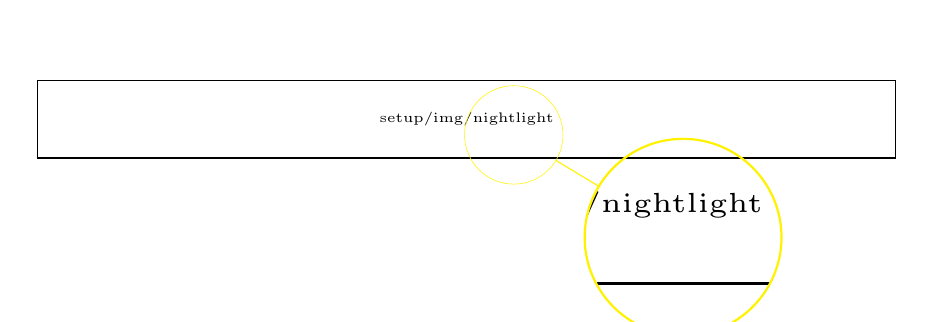
\begin{tikzpicture}[spy using outlines={circle,yellow,magnification=2,size=2.5cm, connect spies}]
\node{\pgfimage[width=0.9\columnwidth]{setup/img/nightlight}};
\spy on (0.6,-0.2) in node [left] at (4,-1.5);
\end{tikzpicture}
\vspace{-0.2cm}
\caption{\newline Sample of night-time luminous intensity satellite image~\cite{kyba2017artificially}. Magnification from Nigeria to Mozambique.
This composite image, shows a global view of Earth at night, compiled from over 400 satellite images. The nighttime light data (2017) was recorded by the Defense Meteorological Satellite Program (DMSP) in the National Geophysical Data Center (NGDC), a part of NOAA. Image Credit: NASA/NOAA.}
\label{fig:sample_of_night_light}
\end{figure}


\section{Problem}
Using just the survey data to predict poverty is time consuming and expensive. Due to lack of transportation and resources, performing such surveys and reaching each and every household is not feasible. With such an anonymous data how can one perform the analysis to determine the poverty of a region?

%Use acronyms:
%The \ac{NOAA} is very nice. It is a \ac{NOAA}

\section{Purpose}
 The project illustrates a methodology to determine the poverty of selected regions using satellite imagery thus helping the nations to take required measures to improve the economic situation. The agricultural improvements can be done in different regions of the nations. Loans can be provided to the needy depending on the situations from the Fintech groups. This work helps the \ac{NGO}s and Governments to grant resources to help these under developed nations by analysing the poverty data.


\section{Goal}
The goal of this project is to build an efficient model which can predict the socioeconomic status of different countries using remote sensing, survey data and google maps.
% The results show the performance analysis of the the models built, based on the correlation between the actual wealth as observed in the survey data and the wealth index predicted by the model. The predicted wealth is mapped on a heat map for visualizing the wealth distribution of the particular regions.

\section{Benefits, Ethics and Sustainability}
If proper measures are taken, both the government and the people get benefited from this work. The per capita income increases and the livelihood of the people becomes better.


\section{Methodology}

This research focuses on the countries in the African continent.
The proposed model is depicted by the flow diagram shown in Fig.~\ref{fig:proposed_model}. It subsumes three stages of core operations: data collection and pre-processing, transfer learning, and training and prediction. The following subsections elaborate each of the stages.



\begin{figure*}[h!]
\centering
  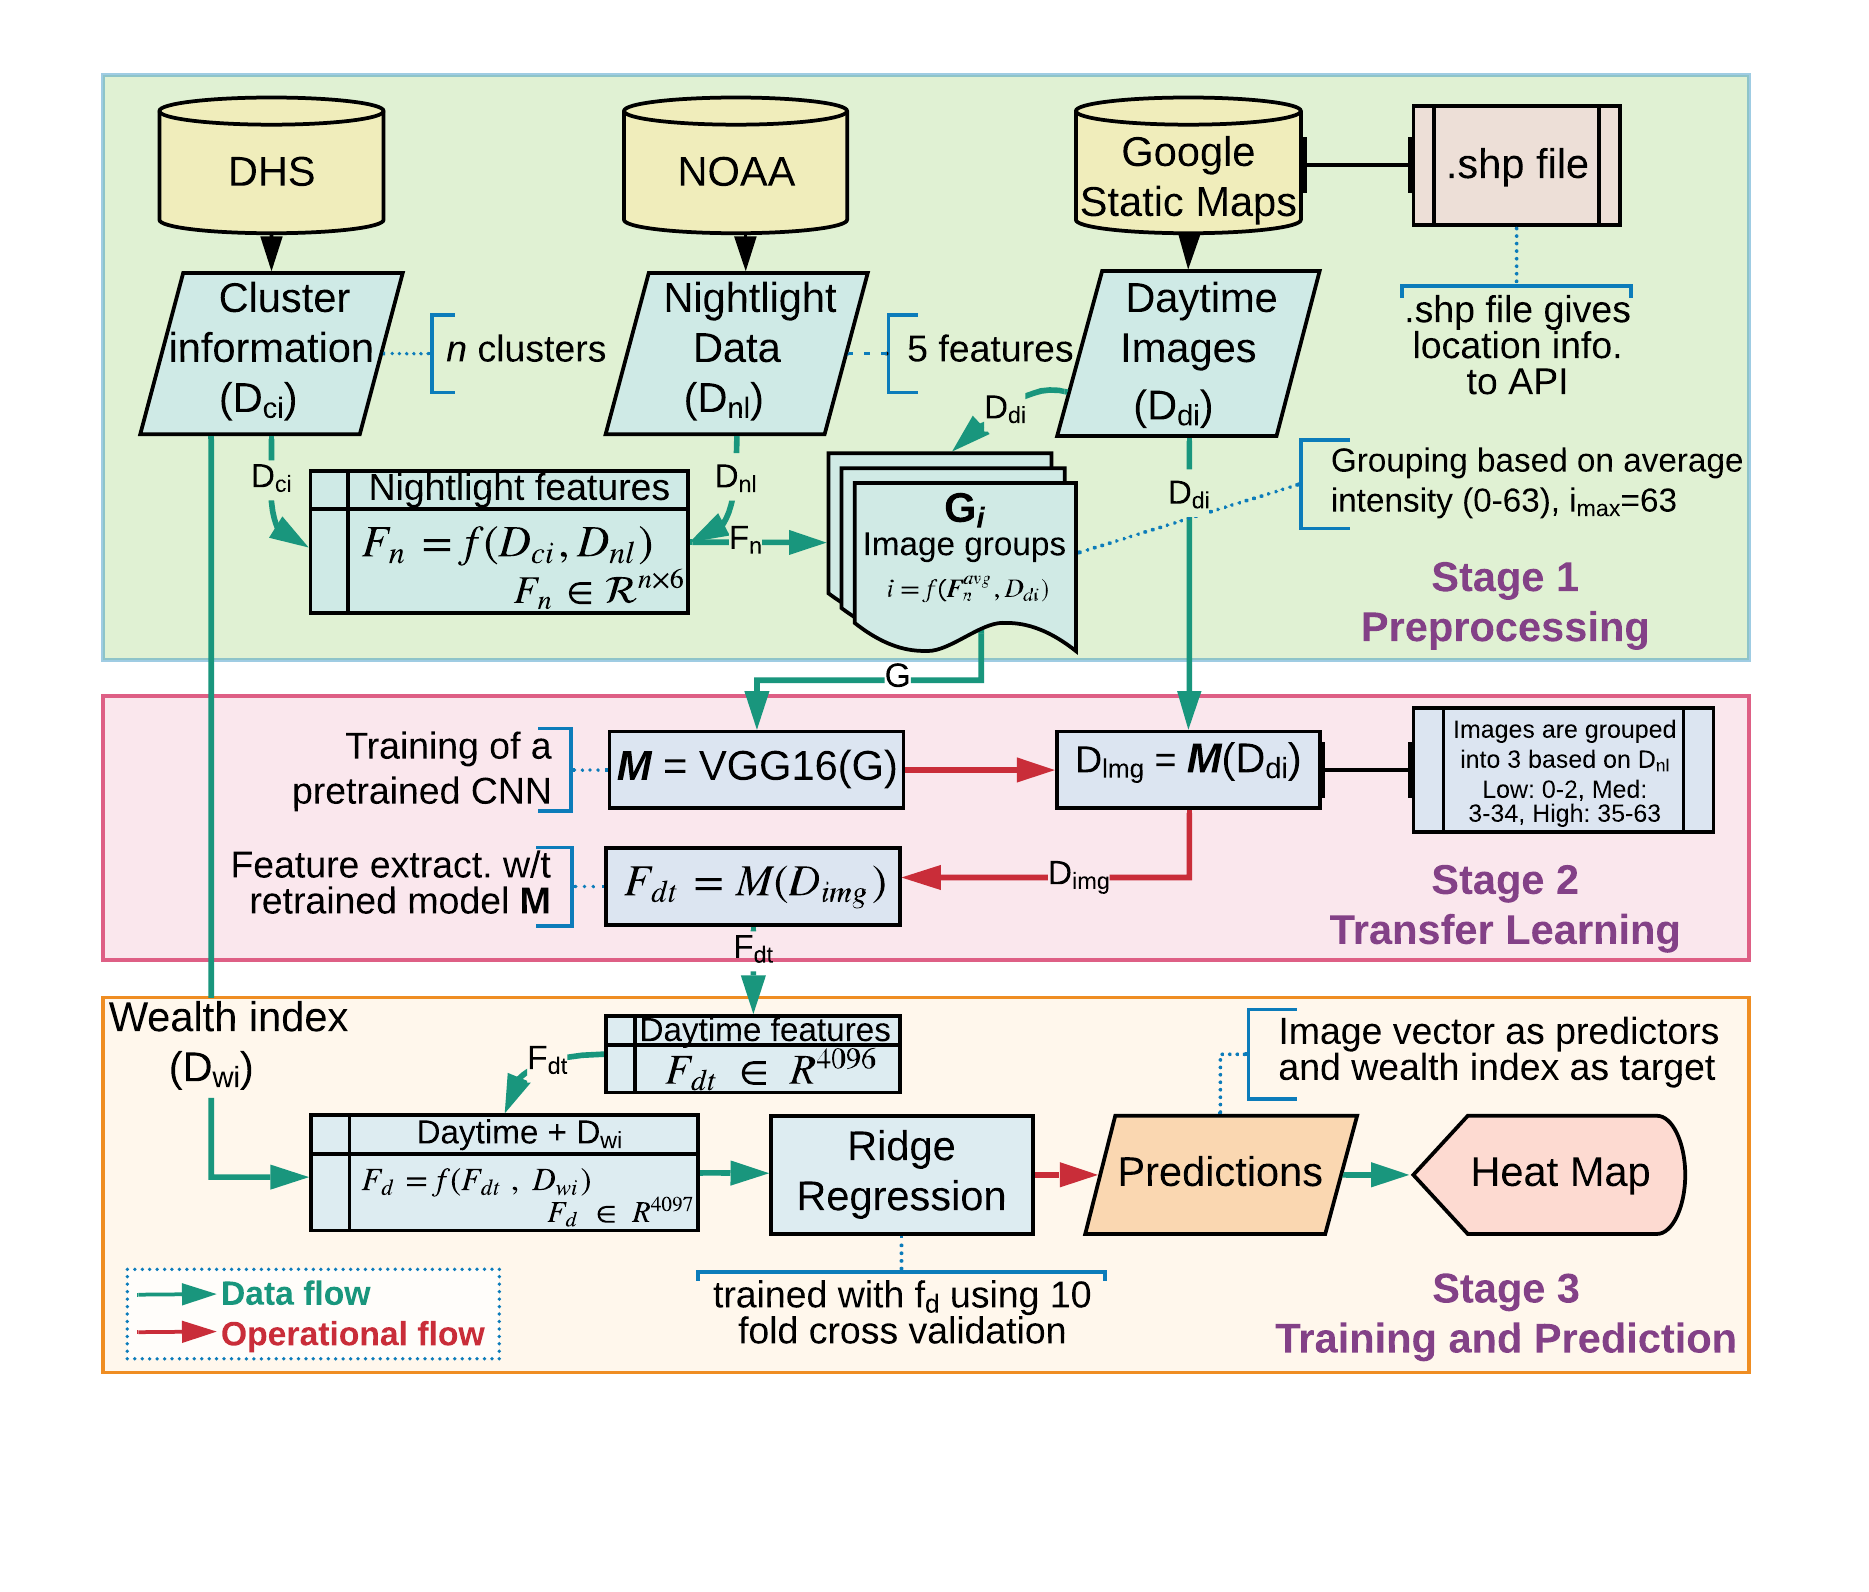
\includegraphics[width=0.99\textwidth]{setup/img/projectfinalflowchart.png}
  \caption{The operational flow of the proposed solution for socioeconomic prediction.}
  \label{fig:proposed_model}
  \centering
\end{figure*}

  


\subsection{Stage 1: Data collection and Preprocessing}
This research focuses on the countries in the African continent, such as, Rwanda, Madagascar, Mozambique, and Nigeria. 
The reason behind choosing these countries is that the majority of the population are still without electricity and the availability of electricity has always been a good representation of the economic status of a region. For the aforesaid regions the following data are collected: NOAA, DHS, and Google Static Maps.

The DHS consists of household records, which includes location information and socioeconomic variables of a particular cluster. We retrieve the household cluster information (latitude, longitude) and the geographic data (shape file) of the particular country selected from DHS. The shape file defines the region boundaries (nation, province, districts etc.). Secondly, NOAA consisting of a high definition raster file, which holds all the nightlight information from which the nighttime satellite images are extracted. The features in the nightlight data are Min, Max, Median, Mean, Standard deviation. Thirdly, Google Static Maps, from which the Daytime satellite images are downloaded using the sector boundary shape file as an input for locations to the API. Basic image features are extracted from the daylight images (simple image metrics). These features are merged with \ac{DHS}, and the regression score is considered in order to test whether they can be used to predict the wealth index. We extract the nightlight features, which contains concatenated features of cluster information and nightlight data with the help of \ac{GDAL} (Geospatial Data Abstraction Library) which is used to read and write the raster and geospatial data formats. We group the satellite images based on average nightlight intensities ($0$-$63$), where $0$ being the lowest intensity and $63$ being the highest intensity.


\subsection{Stage 2: Transfer Learning}

There are only several hundred consumption data points or properties in each country to be used as labelled training examples, it cannot be precisely trained on a broad Convolutional Neural Network (CNN)-based model to estimate such outcomes from satellite images. 
% We do not have enough data. 
To counter the data shortage, we adopt the transfer learning method. Transfer learning enables one to use the knowledge gained from a proxy task into performing a related actual task~\cite{8122666}, in our case the proxy task being the classification based on the abundantly available nightlight data and the actual task being the feature extraction from the daytime images.

To do this, first a \ac{CNN} is trained on a task of high intensity night light estimation. Here, we fine-tune a previously trained VGG 16 on ImageNet to estimate night-time light intensity at different locations, according to the corresponding daytime satellite images. 
% The CNN is used for a classification task where the daylight images are classified into three classes based on night light intensity low, medium, and high.
Due to the global availability of night light data at a resolution of $1 km$, the inputs are $400 \times 400$ pixel daytime satellite images from Google Static Maps at zoom level $16$, which approximately corresponds to $1~km^2$. The day time images are from the year 2019 and the high resolution nightlight image used is from 2017. After the \ac{CNN} model has been trained to classify the images based on the intensity of nightlight into three classes: low (0-2), medium (3-34), and high (35-63), we use this model as a daytime satellite image feature extractor from every cluster that consists of $m$ number of layers by discarding the last layer of the \ac{CNN} model which is the nightlight classification layer. Thus, a cluster is to have a feature vector $\mathbf{F}^c_{dt} \in \mathbb{R}^{m\times 4096}$. This will be further processed by a dimensionality reduction operator $\myfunc{g}$, like:
\begin{equation}
    \mathbf{F}^c_{dt} = \myfunc{g}(\mathbf{F}^c_{dt}), 
    \label{eqn:avg_op}
\end{equation}
where a country may have $C$ number of cluster with a cluster index, $c={1,...,C}$ and $\myfunc{g}$ is a row-wise average operation. Consequentially, a cluster $c$ will have a daytime satellite image feature representation w.r.t night-time luminous values, as $\mathbf{F}^c_{dt} \in \mathbb{R}^{4096}$.

\subsection{Stage 3: Training and Prediction}

This is the stage where the training and predictions take place. Wealth index to corresponding daytime features extracted using the \ac{CNN} re-trained on Nightlight features and is predicted using a ridge regression model. We have conducted trials in which our training labels have been randomly adjusted so that every training example has a randomly paired image vector and wealth label. Each trial tested on a $10$-fold or a $5$-fold cross-validation frame regression model, again selecting regularisation variables in a nested cross-validation mode and after that the image feature dimension is reduced to $100$ using \ac{PCA}. We are plotting the \( R^2\) distribution based on the nightlight intensities and cluster wealth. Using the extracted features and the predicted wealth index, we plot the heat maps. The heat maps show the wealth distribution concluding the Socioeconomic status of the country.





\section{Stakeholders}
Sree Teja Varma Buddaraju, Ananya Bardhan, Ramya Sri Boddu, Simranjit Kaur, Thangarajah~Akilan,~\IEEEmembership{Member,~IEEE}

%\section{Delimitations}
%Explain the delimitations. These are all the things that could affect the study if they were examined and included in the degree project. 
%Use references!

\section{Outline}
The rest of the report is structured as follows:  
\begin{itemize}
    \item Chapter 2 describes the background which is the related work of this work.
    \item Chapter 3 describes the methodologies and methods. It includes information about Ridge Regression, Evaluation matrix and Data sets used for this project.
    \item Chapter 4 describes the work done in this project. It discusses about the impact of data normalization, sanity tests performed, Domain-Specific and Cross-Domain analysis and comparisons between Ridge, Linear and Lasso Regressions.
    \item Chapter 5 describes the results obtained.
    \item Chapter 6 describes the conclusions and discuses the future work.
\end{itemize}
  

\chapter{Theoretical Background}
% \thispagestyle{fancy}

\section{Overview}
This chapter provides the literature review of the project. It discusses about various papers related to this work. Various methods that have been used to predict poverty previously are compared with this work. Remote sensing techniques that have been used to do other experiments are discussed.

\section{Related Work}
In the past, researchers have worked on various strategies to estimate poverty distribution within different countries. Detailed measurements of the economic characteristics of a region have a great impact on both science and strategy. The surveys conducted are based on these policies to make decisions on the allocation of scare resources to track the development towards improving human lives.

Combining the survey data, remote sensing data and new machine learning techniques, researches have been performed on various tasks such as poverty prediction, urban planning, crop yield prediction~\cite{piaggesi2019predicting}. 

In~\cite{jean2016combining}, the authors proposed a transfer learning methodology, where nightlight intensities are used as an intermediate proxy to map poverty in five African countries. When given the inexact data about both daytime imagery and the position of clusters, their models outperform. The proposed work is a modification of~\cite{jean2016combining} restricting to fewer data sets and other African countries. 

In~\cite{perez2017poverty}, have trained a deep neural network to predict poverty from various satellite images without proxies and used other types of remote sensing data for the same task. Other works from~\cite{chen2006remote} analyze the temperature distribution and changes within the city by extracting bare land from satellite images to show its impact on the socioeconomic development.

The work from~\cite{piaggesi2019predicting} shows that they have worked on a similar model like~\cite{jean2016combining}, additionally checking the feasibility of predicting household income of various municipality levels in a city in the USA.

Another work in~\cite{munyati2014inferring}, two high resolution satellite imagery from 2001 and 2010 have been used to examine three socio-economic variables such as main dwelling, toilet facilities and energy resources for cooking. They targeted the image data from 2001 StatsSA census and the new images from 2011 census.They used spatial enhancement and used nearest neighbour resampling algorithm. The image subsets were then used to study the suburban areas with more prominence.

In~\cite{ghosh2013using}, they predict the \ac{GDP} using nightlight images from \ac{NOAA}, \ac{EOG} and the \ac{NGDC}. Considering four countries- U.S., China, Mexico and India. The sum of light intensities and official \ac{GDP} values were regressed. And by using the ratios and sum of lights the value for each  administrative area were predicted.


Inline with this work, the following regions have been analyzed in the past:
\begin{itemize}

\item Nairobi- Algorithms were built to process satellite images and make assumptions on the economic state of slums based on the reflective index of the roofs and night light images\cite{zhao2016spectral}.
\item USA- Nightlight images and daytime images were used to observe the density of settlement and the fall line to set up coasts close by for reducing shipment costs.
\item Indonesia- Study of deforestation and 1997 wildfires \cite{xie2016transfer}. 

\end{itemize}

There is no systematic study of the regions this work focuses on to compare the proposed model results with existing model results.

\section{Summary}
There have been various researches conducted in the past. Remote sensing and machine learning are the common domains chosen for these experiments. Remote sensing is used for poverty prediction, urban planning, crop yield prediction, temperature distribution etc. Aided by machine learning, researchers have put their interest to perform experiments to study deforestation, wild fires, population settlements,   Our work is inspired from~\cite{jean2016combining} leading us to predict poverty using satellite imagery, survey data and night-light data. 
\chapter{Engineering-related content, Methodologies and Methods}
% \thispagestyle{fancy}

\section{Overview}
This chapter describes the experimental methodology and techniques that we use to get our results.


\section{Ridge Regression}
It is a linear regression model which imposes square penalties on the linear coefficient dimensions. As the image features have a large size $(d=4096)$ regularisation helps to keep relatively small training sets from being overly matched. In an internal cross-validation circuit, the choice of a regularisation parameter has been made to preserve the integrity of the hold-out test details.
The parameters of ridge regression are: \(alpha, ~fit~intercept, ~normalize, ~copy~X, ~max~iter,~tol\) and \(solver\). \(~Fit~intercept, ~normalize,\) and \(~copy~X\) are Boolean values. \(Alpha\) is the regularization strength. \(Fit~intercept\) is used to know whether to calculate the intercept or not. The regressor will be normalized before regression by subtracting the mean and divided by the l2-norm when \(Normalize\) is \(true\). The regressor may be copied or overwritten depending on whether \(copy~X\) is \(true\) or \(false\) respectively. These parameters are altered along with the number of splits $(10~or~5)$ and the obtained \(R^2\) scores are tabulated.

\section{Evaluation Metrics}
The following are used to evaluate the performance of the proposed model:
\begin{itemize} 
\item \(R^2\) Score: It provides an indication of fitness and therefore a measure of how well the unseen samples are likely to be predicted by the model due to the proportion of explained variance($y$). The best possible score is $1.0$ and may be negative (because the model may be worse off arbitrarily). A constant model that always predicts the expected value of $y$, regardless of the input features, would have an \(R^2\) value of $0.0$. If $\hat{y}_i$ is the predicted value of the \(i\)-th sample and $y_i$ is  is the corresponding true value for total \(n\) samples, the estimated \(R^2\) is defined as in \ref{eq:r_2}.

\begin{equation}
    R^2(y, \hat{y}) = 1 - \frac{\sum_{i=1}^{n} (y_i - \hat{y}_i)^2}{\sum_{i=1}^{n} (y_i - \bar{y})^2},
    \label{eq:r_2}
\end{equation}
where $\bar{y} = \frac{1}{n} \sum_{i=1}^{n} y_i$, and $\sum_{i=1}^{n} (y_i - \hat{y}_i)^2 = \sum_{i=1}^{n} \epsilon_i^2$.\\

\item Mean Square Error(MSE): the mean squared error or mean squared deviation of an estimator measures the average of the squares of the errors—that is, the average squared difference between the estimated values and the actual value. MSE is a risk function, corresponding to the expected value of the squared error loss. If $y_i$ is the set of actual values and $\hat{y}_i$ is the set of predicted values from a sample of $n$ points.The MSE is defined as in \ref{eq:MSE}
\begin{equation}
    MSE =  \frac{1}{n} \sum_{i=1}^{n} (y_i - \hat{y}_i)^2
    \label{eq:MSE}
\end{equation}
i.e., MSE is the mean $\frac{1}{n} \sum_{i=1}^{n}$ of the squares of errors $(y_i - \hat{y}_i)^2$.  

\end{itemize}
\section{Datasets}

The data used in this work are obtained from the following sources. 
\begin{itemize}
\item DHS\footnote{https://dhsprogram.com/data/}: We obtain the survey data from Demographic Health Survey website which is used as a source of household cluster information, cluster locations and wealth index; Nigeria - $867$ clusters, Mozambique - $225$ clusters, Rwanda - $492$, Madagascar - $375$ clusters.
\item NOAA\footnote{https://ngdc.noaa.gov/eog/dmsp/downloadV4composites.html}: We obtain a high definition raster graphic file (.tiff) from National Oceanic and Atmospheric Administration which contains the world map with all the nightlights and provides us with all the nightlight information.

\item Google Static Maps\footnote{https://cloud.google.com/maps-platform/}: We employ the google static maps API to obtain all the daytime images as required by giving the boundary shape of of each country as a input. All the images downloaded are of $400 \times 400$ at a $1km^2$ range. The following are the number of images considered for each country : Rwanda- $50,532$ images, Mozambique- $23,778$ images, Madagascar- $38,587$ images, Nigeria- $89,214$

\end{itemize}

\begin{table}[h!]
\setlength\tabcolsep{4.5pt}
\caption {Summary of the Datasets} \label{tab:1} 
\begin{center}
\begin{tabular}{|c|c|c|c|c|} 
\hline
Dataset & Rwanda & Madagascar & Mozambique & Nigeria    \\
\hline
DHS (clusters) & 492 & 375 & 225 & 867 \\ 
Google Static Maps & 50,532 & 38,587 & 23,778 & 89,214\\ 
NOAA & 1 & 1 & 1 & 1 \\
\hline
\end{tabular}
\end{center}

\end{table}



\section{Summary}
Ridge regression is a linear regression model which imposes square penalties on the linear coefficient dimensions. \(R^2\) score and Mean Square Error are considered for evaluating the proposed model. \(R^2\) score tells how likely the unseen samples can be predicted by the model. Mean Square Error is the mean of the squares of errors. The datasets used in this work are the household recode data from DHS which also gives the cluster locations and wealth index.A night-light image of the world map as a high definition raster graphic file from NOAA. Day time satellite images from Google Static Maps. These day time images are obtained after specifying the boundary shape file of each country.

\chapter{The work}
\section{Overview}
This chapter mainly focuses on the results of the work. It consists of the qualitative analysis. This includes all the major experiments which have been tabulated with their values. 

\section{Quantitative Analysis}
All the previous work conducted in this domain was comprised of different countries and additional datasets. Hence, it was very difficult to compare the experimental results of this approach with any other work, because of the variance of datasets and consideration of other countries to conduct the analysis. For each country, we evaluated regression models for predictions with either $5$ or $10$-fold cross-validation. The results are tabulated in Table~\ref{tab:1} - \ref{tab:4} with various hyper parameter settings. 


\newline
\section{Sanity Test}

\begin{table}[h!]
 \caption{Retrained CNN Model of Rwanda}
 \label{tab:3} 
\begin{center}
\begin{tabular}{|c|c|c|c|c|}
\hline
Trails & Epochs & Train Batch & Test Batch & $R^2$    \\
\hline\hline
1 & 10 & 1700 & 146 & 0.652 \\
2 & 10 & 8000 & 1700 & 0.705 \\
\hline\hline
\end{tabular}
\end{center}
\end{table}

In {Table~\ref{tab:3}},
\newline the training and testing sample sizes were relatively small compared to the actual data. These $R^2$ scores were obtained from the data which was not shuffled. Two trails were conducted and only $10$ epochs were executed for each trail. Trail $1$ has $0.652$ $R^2$ score and as the sample sizes are increased in trail $2$, the $R^2$ score is increased. Some of the data got overlapped while performing these experiments resulting in these $R^2$ scores. Other experiments were carried out with shuffled data on different countries and the following are the results.


\section{Domain-Specific Performance}
In {Table~\ref{tab:4}}, these results were obtained using bigger train and test sample sizes. It was executed for $50$ epochs for each of the four countries. It is observed that using these sample sizes gives a reasonable \(R^2\) values and helps to achieve a high prediction value to generate a distinguishable heat map. We have three kinds of labels which include the \(R^2\) values and number of clusters of each of the four countries and also the values after merging the clusters of more than one country and we observe that even though combining Rwanda and Nigeria did not give a suitable \(R^2\), but when Rwanda, Nigeria and Mozambique were combined, then a high \(R^2\) value was obtained. These are the \(R^2\) values after prediction of the wealth index of the countries, Rwanda, Mozambique, Nigeria and Madagascar.These experiments were conducted using the best set of hyper parameters as obtained from Table~\ref{tab:1} and Table~\ref{tab:2}, which gave a high value of \(R^2\) before and after normalization. 

\begin{table}[h!]
 \caption{Domain-specific Analysis}
 \label{tab:4} 
\begin{center}
\begin{tabular}{|c|c|c|c|c|c|}
\hline
Country & Epochs & Train size & Test size & \(R^2\) score & clusters \\
\hline\hline
Madagascar & 50 & 8000 & 2000 & 0.732 & 375 \\
Nigeria & 50 &  16000    &  4000 & 0.456 & 867 \\
Rwanda & 50 & 24000 & 6000 & 0.752 & 492 \\
Mozambique & 50 &  8000    &  2000 & 0.762 & 225\\

 
\hline \hline
\end{tabular}
\end{center}
\end{table}


\begin{table}[h!]
 \caption{Mean Square Error}
 \label{tab:9} 
\begin{center}
\begin{tabular}{|c|c|c|}
\hline
Country & 5-Fold & 80:20    \\
\hline\hline
Rwanda & 0.129 & 0.225 \\
Mozambique & 0.216 & 0.211 \\
Madagascar & 0.203 & 0.232\\
Nigeria & 0.281 & 0.304\\
\hline\hline
\end{tabular}
\end{center}
\end{table}

{Table~\ref{tab:9}}, shows the \ac{MSE} for both the K-fold and 80:20 train and test data spilt. Here, it can be observed that error values is less with the K-fold and hence it is used in the model.







\section{Cross-Domain Analysis}

\begin{table}[h!]
 \caption{Merged Domain Performance Analysis}
 \label{tab:7} 
\begin{center}
\begin{tabular}{|l|c|c|c|c|c|}
\hline
\hspace{1cm}{Merged Domain}   & clusters & \(R^2\) score   \\
\hline\hline
Rwanda, Nigeria  & 1359 & 0.634   \\
Rwanda, Nigeria, Mozambique  & 1584 & 0.782  \\
\hline\hline
 
\end{tabular}
\end{center}
\end{table}

In Table~\ref{tab:7}, the models of different countries were merged, and it can be seen that the \(R^2\) score for the combined model of Rwanda and Nigeria is less, as due to Nigeria's score the total performance decreases. But when models of Rwanda, Nigeria and Mozambique are combined, it gives a higher score and performs better.


\section{Comparision with other Regession Models}

\begin{table}[h!]
 \caption{Results using differnt rigression models}
 \label{tab:8} 
\begin{center}
\begin{tabular}{|l|c|c|c|c|c|}
\hline
Country & clusters & ridge & lasso & linear   \\
\hline\hline
Rwanda  & 492 & 0.752 & 0.742 & 0.739  \\
Mozambique & 225 & 0.762 & 0.757 & 0.720\\
Madagascar & 375 & 0.732 & 0.729 & 0.720\\
Nigeria & 867 & 0.456 & 0.427 & 0.359\\

\hline\hline
 
\end{tabular}
\end{center}
\end{table}
In Table~\ref{tab:8}, the different models of regression is been compared, and it can be found that among Linear, Lasso and Ridge Regression, the Ridge Regression gives the better \(R^2\) scores. Therefore, we go forward with Ridge Regression to get the results.

\section{Summary}
The experimental results are tabulated. From these tables it can be observed that of all the regression models, Ridge regression has better performance. When considering the time consumption for various regression models, Ridge takes optimal time to do the computation. 
\chapter{Results}

\section{Overview}
This chapter shows the results obtained after performing computations on the datasets. The plot and heat maps are generated to get a better visualization of the results obtained.

\section{Qualitative Analysis}
The following are the results we obtain in the form of graph for Rwanda and heat maps of countries Rwanda, Mozambique, Nigeria and Madagascar. These are the results obtained using the model mentioned in the report.


\begin{figure}[h!]
\centering
  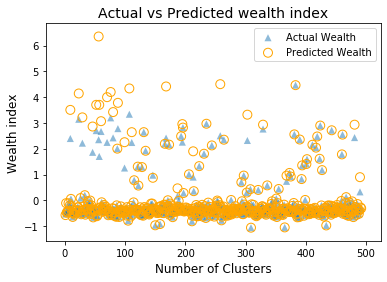
\includegraphics[width=8cm]{setup/img/actvspredwlth.png}
  \newline
  \caption{Actual wealth vs predicted wealth of Rwanda.}
  \label{fig3}
  \centering
\end{figure}




\begin{figure*}[!ht]
    \hspace{3cm} Input: Sample Day-time satellite images
    \newline
    \newline
     \centering
     %----day-time inputs--------------
     \begin{subfigure}[t]{0.22\textwidth}
         \centering
         \setlength{\unitlength}{0.1\textwidth}
         \begin{picture}(10,9)
         \put(0,0){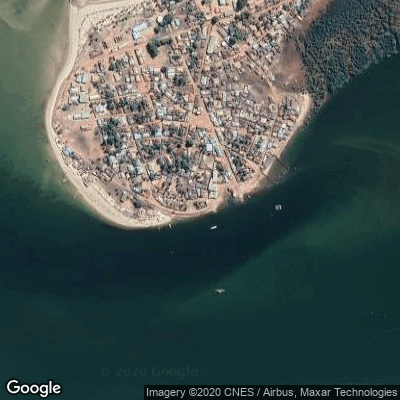
\includegraphics[trim={0.5cm, 0cm, 0cm, 2.25cm}, clip, width=\columnwidth]{setup/img/Madagascar_day.png}}
         \color{yellow}
         \put(0.0,0.5){{-16.104434,45.328354}}
         \end{picture}
        %  \caption{Madagascar}
         \label{fig:y equals x}
     \end{subfigure}
     \hfill
     \begin{subfigure}[t]{0.22\textwidth}
         \centering
         \setlength{\unitlength}{0.1\textwidth}
         \begin{picture}(10,9)
         \put(0,0){
\includegraphics[trim={0.5cm, 0cm, 0cm, 2.25cm}, clip, width=\columnwidth]{setup/img/nigeria_day.png}}
         \color{yellow}
         \put(0.0,0.5){{9.145108,7.316459}}
        %  \caption{Nigeria}
         \end{picture}
         \label{fig:five over x}
     \end{subfigure} 
     \hfill
    \begin{subfigure}[t]{0.22\textwidth}
         \centering
         \setlength{\unitlength}{0.1\textwidth}
         \begin{picture}(10,9)
         \put(0,0){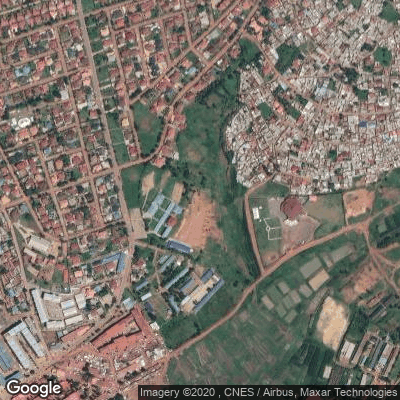
\includegraphics[trim={0.5cm, 0cm, 0cm, 2.25cm}, clip, width=\columnwidth]{setup/img/Rwanda_day.png}}
         \color{yellow}
         \put(0.0,0.5){{-1.920349,30.074494}}
         \end{picture}
        %  \caption{Rwanda}
         \label{fig:five over x}
     \end{subfigure}
     \hfill
     \begin{subfigure}[t]{0.22\textwidth}
         \centering
         \setlength{\unitlength}{0.1\textwidth}
         \begin{picture}(10,9)
         \put(0,0){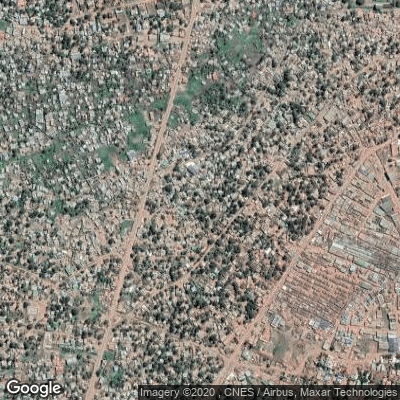
\includegraphics[trim={0.5cm, 0cm, 0cm, 2.25cm}, clip, width=\columnwidth]{setup/img/Mozambique_day.png}}
         \color{yellow}
         \put(0.0,0.5){{-19.13401772,33.48299979}}
         \end{picture}
        %  \caption{Mozambique}
         \label{fig:three sin x}
     \end{subfigure}
     \hfill

    %----predicted heat-map--------------
    

     \centering
     \begin{subfigure}[t]{0.22\textwidth}
         \centering
         \setlength{\unitlength}{0.1\textwidth}
         \begin{picture}(10,9)
         \put(0,0){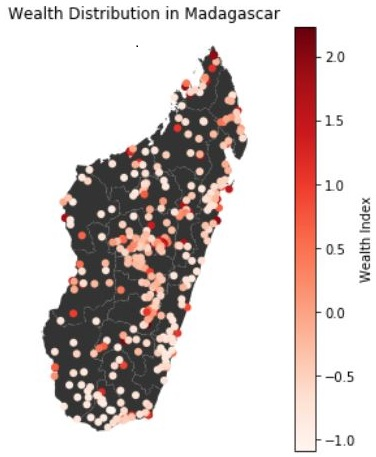
\includegraphics[trim={0.5cm, 0.5cm, 2.0cm, 1.0cm}, clip, height=3.6cm]{setup/img/Madagascar.JPG}}
         \color{yellow}
         \put(1.5,6.3){\vector(1,2){2.45}}
         \end{picture}
         %\caption{Madagascar}
         \label{fig:y equals x}
     \end{subfigure}
     \hfill
     \begin{subfigure}[t]{0.22\textwidth}
         \centering
         \setlength{\unitlength}{0.1\textwidth}
         \begin{picture}(10,9)
         \put(0,0){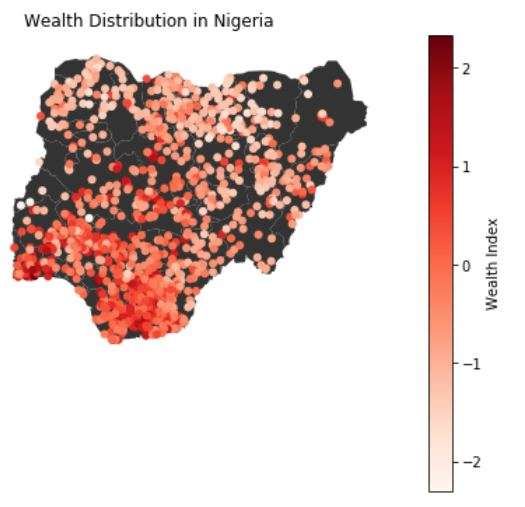
\includegraphics[trim={0.1cm, 3.0cm, 2.5cm, 1.0cm}, clip, height=3.6cm]{setup/img/Nigeria.JPG}}
         \color{yellow}
         \put(4,4.5){\vector(1,2){3.35}}
         \end{picture}
         %\caption{Nigeria}
         \label{fig:five over x}
     \end{subfigure} 
     \hfill
    \begin{subfigure}[t]{0.22\textwidth}
         \centering
         \setlength{\unitlength}{0.1\textwidth}
         \begin{picture}(10,9)
         \put(0,0){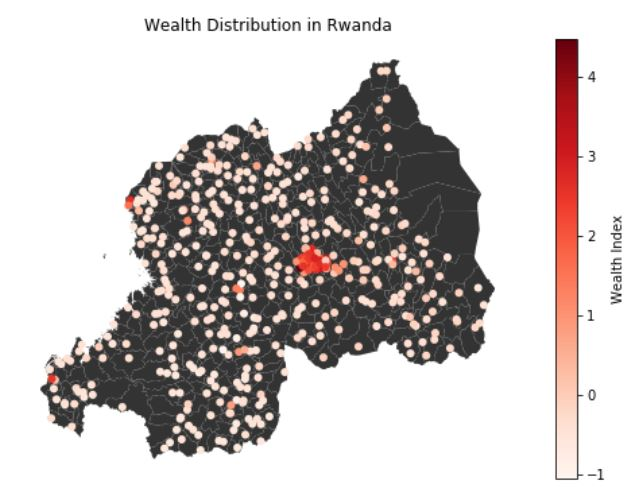
\includegraphics[trim={0.5cm, 0.5cm, 2.5cm, 1.0cm}, clip, height=3.6cm]{setup/img/rwanda.JPG}}
         \color{yellow}
         \put(6,4.5){\vector(1,2){3.35}}
         \end{picture}
         %\caption{Rwanda}
         \label{fig:five over x}
     \end{subfigure}
     \hfill
     \begin{subfigure}[t]{0.25\textwidth}
         \centering
         \setlength{\unitlength}{0.1\textwidth}
         \begin{picture}(10,9)
         \put(0,0){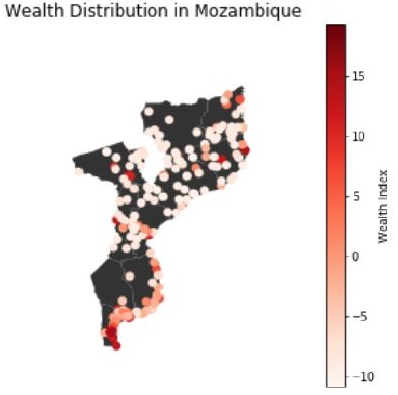
\includegraphics[trim={0.5cm, 0.5cm, 0.1cm, 1.5cm}, clip, height=3.6cm]{setup/img/Mozambique.JPG}}
         \color{yellow}
         \put(2.5,3.80){\vector(1,2){3.05}}
         \end{picture}
         %\caption{Mozambique}
         \label{fig:three sin x}
     \end{subfigure}
     \hfill

     %---- actual heat-map--------------
     \hspace{3cm} Output: Predicted wealth index heat map
     \newline \newline
     \newline
     \begin{subfigure}[t]{0.22\textwidth}

         \centering
         \setlength{\unitlength}{0.1\textwidth}
         \begin{picture}(10,9)
         \put(0,0){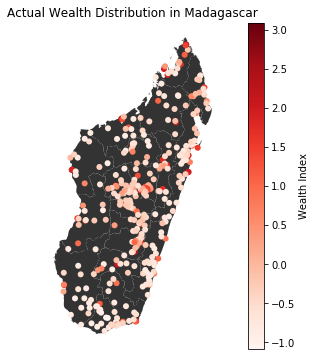
\includegraphics[trim={0.5cm, 0.5cm, 2.5cm, 1.5cm}, clip, height=3.6cm]{setup/img/Act_Madagascar.png}}

         \end{picture}
         \caption{Madagascar}
         \label{fig:y equals x}
     \end{subfigure}
     \hfill
     \begin{subfigure}[t]{0.22\textwidth}
         \centering
         \setlength{\unitlength}{0.1\textwidth}
         \begin{picture}(10,9)
         \put(0,0){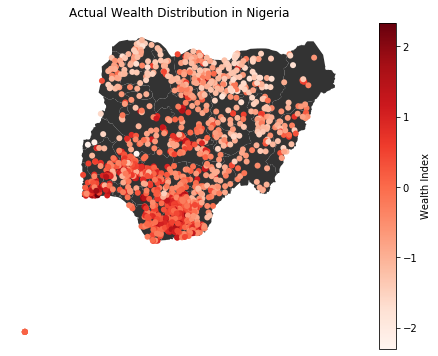
\includegraphics[trim={2.5cm, 2.5cm, 2.5cm, 1.5cm}, clip, height=3.6cm]{setup/img/Act_Nigeria.png}}
         \end{picture}
         \caption{Nigeria}
         \label{fig:five over x}
     \end{subfigure} 
     \hfill
     \begin{subfigure}[t]{0.22\textwidth}
         \centering
         \setlength{\unitlength}{0.1\textwidth}
         \begin{picture}(10,9)
         \put(0,0){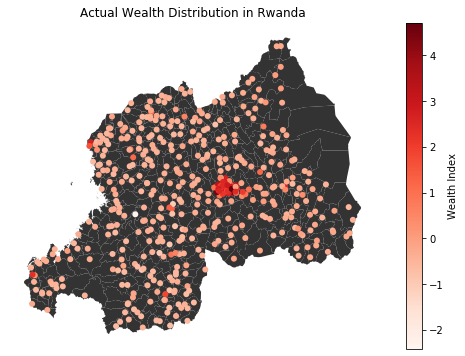
\includegraphics[trim={0.5cm, 0cm, 2.5cm, 1cm}, clip, height=3.6cm]{setup/img/Act_Rwanda.png}}

         \end{picture}
         \caption{Rwanda}
         \label{fig:five over x}
     \end{subfigure}
     \hfill
     \begin{subfigure}[t]{0.22\textwidth}
         \centering
         \setlength{\unitlength}{0.1\textwidth}
         \begin{picture}(10,9)
         \put(0,0){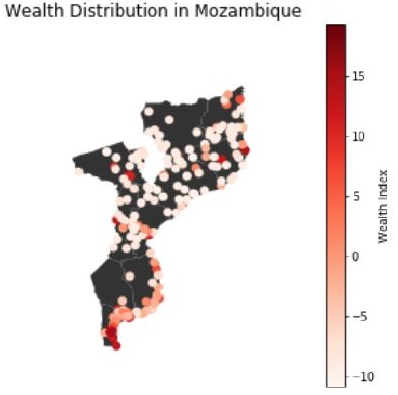
\includegraphics[trim={0.5cm, 0cm, 0cm, 1.25cm}, clip, height=3.6cm]{setup/img/Act_Mozambique.JPG}}
         
         \end{picture}
         \caption{Mozambique}
         \label{fig:three sin x}
     \end{subfigure}
     \hfill
     \newline
     \newline
     \newline
    \hspace{3cm} Actual wealth index heat map
     
     \caption{The inputs (day-time satellite images) taken from satellite CNES/Airbus of Maxar Technologies, 2019 and the predicted wealth index heat-maps of the countries: Madagascar, Nigeria, Rwanda, Mozambique. The resolution of day-time images is $400\times 400$ $dpi$.}
     \label{fig:predicted_hmap}
    
    
\end{figure*}



Fig.~\ref{fig3} compares the actual and predicted wealth index w.r.t. the number of clusters of the country, Rwanda. This scatter plot shows the difference between the original wealth and the model wealth where most of the clusters are below the $0$ wealth index. Moreover, both wealth indexes overlap at most of the clusters indicating no drastic discrepancies. Similar graphs are plotted for other countries. Fig.~\ref{fig:predicted_hmap} shows the day-time satellite images and wealth distribution in a heat map of the countries: Madagascar, Nigeria, Rwanda, and Mozambique. The day-time images here are the samples taken from medium and high-intensity categories to show human settlements of the above-mentioned countries. The corresponding night-light intensities of Madagascar, Nigeria, Rwanda, and Mozambique are $5$, $37$, $62$, and $42$ respectively. The wealth index scale differs for every country. 

\chapter{Conclusion}
In this work, it is found that the daytime satellite images can help to predict wealth distributions resulting in more accurate results as expected. As discussed in this paper, due to the data gaps only one source of data sets would be insufficient to predict better results. Both daytime and nighttime imagery is thus used. The household recode data has been used for verification. Another feature of this model is that it can perform on any resolution of satellite images but usage of high resolution images is recommended to achieve desired outputs. It is a cheaper, high performing and reliable source to fill the data gaps from the survey data using the widely available satellite images. It is not feasible for regions with very little or no survey data to use a similar approach as the model is highly dependable on previous data for training and predictions. Ridge regression models are used for this experiment because of its lesser time consumption and greater $R^2$ scores when compared with Lasso and Linear regressions. To compare the results obtained with existing models, there were no experiments performed on all the countries chosen for this work.  


%\section{Discussion}

\section{Future Work}
For the future work, we plan on using the models trained on one region with the other region's data to observe how they perform and also try to observe the performance of the models when trained on multiple regions at once.

\section{Final Words}
These predictions can help with research and analysis that can help many organizations and governments make better decisions on where to devote their time and resources efficiently in order to help enhance the economical standards of particular undeveloped regions.




% \include{content}

\newpage
\addcontentsline{toc}{chapter}{References}
\printbibliography


\newpage
\appendix
\newpage
\etocdepthtag.toc{mtappendix}
\etocsettagdepth{mtchapter}{none}
\etocsettagdepth{mtappendix}{subsection}
\etoctocstyle{1}{Appendix - Contents}
\tableofcontents
\newpage


\chapter{First Appendix}


\section{Impact of Data Normalization}

The following are the experiments performed with data normalization. Table~\ref{tab:1} and table~\ref{tab:2} are the observations before and after normalization respectively. These were the results taken for input data of day-time features obtained after merging the DHS data with day-time images. Table~\ref{tab:3} is built using the results obtained with the input data of day-time images after grouping them into classes low, medium and high. Merging features extracted from the retrained \ac{CNN} model and the wealth index of the clusters as input data the \(R^2\) values obtained and tabulated in Table~\ref{tab:4}.


\begin{table}[h!]

\caption {Ridge Regression before data normalization} \label{tab:1} 
\begin{center}
\begin{tabular}{|c|c|c|c|c|c|} 
\hline
K-Fold & Alpha & Fit intercept & Normalize & Copy X & T(or)F    \\
\hline \hline
10 & 0.752 & 0.725 & 0.752 & 0.725 & TRUE \\ 
10& 0.581 & 0.562 & 0.581 & 0.581 & FALSE \\ 
5 & 0.761 & 0.753 & 0.761 & 0.758 & TRUE  \\ 
5 & 0.758 & 0.758 & 0.761 & 0.758 & FALSE  \\ 
\hline \hline
\end{tabular}
\end{center}
\end{table}

%\centerline{\includegraphics{ref{tab:TABLE I}}}
In {Table~\ref{tab:1}}, $10$ and $5$ fold cross validation were considered for ridge regression before normalization. From the above table, it can be depicted that all the parameters give better \(R^2\) results with $5$ folds. In some cases the \(R^2\) value remains the same even after change in the input parameter. 


\begin{table}[h!]
 \caption{Ridge Regression after data normalization} 
\label{tab:2} 
\begin{center}
\begin{tabular}{|c|c|c|c|c|c|} 
\hline
K-Fold & Alpha & Fit intercept & Normalize & Copy X & T(or)F    \\
\hline\hline
10 & 0.752 & 0.725 & 0.752 & 0.725 & TRUE \\ 
10 & 0.581 & 0.562 & 0.702 & 0.581 & FALSE \\ 
5 & 0.761 & 0.725 & 0.761 & 0.758 & TRUE \\ 
5 & 0.758 & 0.725 & 0.752 & 0.725 & FALSE \\ 
\hline\hline
\end{tabular}
\end{center}
\end{table}

In {Table~\ref{tab:2}}, this is the observation made after conducting normalization using $10$ and $5$ folds. It can also be depicted that the \(R^2\) values were different under some parameters before and after normalization. There was a decrease in the score for $5$ fold after normalization while, the $10$ fold score still varies accordingly.\newline
The parameters giving the best results from Table~\ref{tab:1} and Table~\ref{tab:2} are used to carry on further experiments to give better \(R^2\) scores.

\section{Time Analysis}

\begin{table}[h!]
 \caption{Time Analysis for Rwanda(in sec)}
 \label{tab:10} 
\begin{center}
\begin{tabular}{|c|c|c|c|}
\hline
Country & Linear & Lasso & Ridge   \\
\hline\hline
Rwanda & 0.011 & 0.038 & 0.041 \\
Mozambique & 0.084 & 0.093 & 0.021 \\
Madagascar & 0.078 & 0.079 & 0.019\\
Nigeria & 0.078 & 0.079 & 0.021\\
\hline\hline
\end{tabular}
\end{center}
\end{table}
In {Table~\ref{tab:10}}, the time taken to compute the results using the three regression models can be observed. But the time taken by Ridge Regression is very less compared to the others.

\section{Comparing results from 5-fold cross validation and 80:20 split}

\begin{table}[h!]
 \caption{\(R^2\) Scores: 5-fold Cross Validation}
 \label{tab:10} 
\begin{center}
\begin{tabular}{|c|c|c|c|}
\hline
Country & Linear & Lasso & Ridge   \\
\hline\hline
Rwanda &  0.752 &  0.742 & 0.739 \\
Mozambique &0.762 & 0.757 & 0.749 \\
Madagascar & 0.732 & 0.729 & 0.720\\
Nigeria & 0.686 & 0.627 & 0.609\\
\hline\hline
\end{tabular}
\end{center}
\end{table}

\begin{table}[h!]
 \caption{\(R^2\) Scores: 5-fold Cross Validation}
 \label{tab:10} 
\begin{center}
\begin{tabular}{|c|c|c|c|}
\hline
Country & Linear & Lasso & Ridge   \\
\hline\hline
Rwanda &   0.740 &  0.735& 0.739 \\
Mozambique &0.762 & 0.751 & 0.749 \\
Madagascar &0.745 & 0.729 & 0.720\\
Nigeria & 0.642 & 0.620 & 0.609\\
\hline\hline
\end{tabular}
\end{center}
\end{table}













\section{GitHub Repository}
The GitHub repository for this project:
\newline
https://github.com/SreeTejaVarma/socio-economic-analysis-using-satellite-imagery
\newpage
% This is the last page of the document
\thispagestyle{empty}
\AddToShipoutPictureBG*{%]
    \AtPageLowerLeft{%
        \includegraphics[width=1.0\paperwidth]{setup/img/kth-footer.png}
    }%
}

\PlaceText{20mm}{282mm}{\color{white}\fontsize{12}{0}\sffamily www.kth.se }


\end{document}
